
\documentclass[svgnames]{beamer}

\mode<presentation> {
\usetheme{Warsaw}
}

\usepackage{graphicx}
\usepackage{booktabs}
\usepackage{listings}
\usepackage{color}
\usepackage[lofdepth,lotdepth]{subfig}
\usepackage{fontawesome}
\usepackage{hyperref}

\definecolor{codegreen}{rgb}{0,0.6,0}
\definecolor{codegray}{rgb}{0.5,0.5,0.5}
\definecolor{codepurple}{rgb}{0.58,0,0.82}
\definecolor{backcolour}{rgb}{0.95,0.95,0.92}

\beamertemplatenavigationsymbolsempty


\lstdefinestyle{mystyle}{
    backgroundcolor=\color{backcolour},   
    commentstyle=\color{codegreen},
    keywordstyle=\color{magenta},
    numberstyle=\tiny\color{codegray},
    stringstyle=\color{codepurple},
    %basicstyle=\footnotesize,
    basicstyle=\scriptsize\ttfamily,
    breakatwhitespace=false,         
    breaklines=true,                 
    captionpos=b,                    
    keepspaces=true,                 
    numbers=none,                    
    numbersep=5pt,                  
    showspaces=false,                
    showstringspaces=false,
    showtabs=false,                  
    tabsize=2,
    language=bash
}

\lstset{style=mystyle}

% \newcommand{\SubItem}[1]{
%     {\setlength\itemindent{15pt} \item[-] #1}
% }

%------------
%	TITLE PAGE
%------------

\title[Practical session: Version control, Git, GitHub and GitFlow]{Practical session: Version control, Git, GitHub and GitFlow} \author{Criscely Luj\'{a}n \\ criscely.lujan@ird.fr \\ \and
Nicolas Barrier \\
nicolas.barrier@ird.fr}
\institute[Universit\'{e} Paris-Sud, UMR MARBEC]  
{Universit\'{e} Paris-Sud, UMR MARBEC \\ 
\medskip
\textit{criscely.lujan@ird.fr}
}
\author[Criscely Luj\'{a}n \& Nicolas Barrier]{Criscely Luj\'{a}n\inst{1,2} \\ \vspace{-0.5em} \tiny \emph{\href{mailto:criscely.lujan@ird.fr}{criscely.lujan@ird.fr}} \normalsize \\ \vspace{1em}
                         \and Nicolas Barrier\inst{2}\\  \tiny \emph{\href{mailto:nicolas.barrier@ird.fr}{nicolas.barrier@ird.fr}}}
\institute[shortinst]{\inst{1} Universit\'{e} Paris-Sud, UMR MARBEC \and \inst{2} IRD, UMR MARBEC}

\date{April 11, 2019}

\hypersetup{
    colorlinks=true,
    linkcolor=white,
    urlcolor=blue,
}

\AtBeginSection[]
{
    \begin{frame}
         \hypersetup{linkcolor=black}
        \frametitle{Table of Contents}
                  \tableofcontents[currentsection]
    \end{frame}
}


\begin{document}

%------------
\begin{frame}
\titlepage 
    \vspace{-1em}
\begin{center}

\includegraphics[height=1cm]{img/logo_psud.jpg}
\hspace{1em}

\includegraphics[height=1cm]{img/logo_marbec.png}
\hspace{1em}

\includegraphics[height=1cm]{img/logo_ird.png}
\end{center}
\end{frame}

\section{Git basis (beginners)}


\begin{frame}
\frametitle{GitHub account}

Tips about the name account:

\begin{itemize}
    \item Use your actual name!
    \item Shorter is better than longer!
    \item Be as unique as possible!
    \item Re-use your name from other context, e.g. \faTwitter, \faSlack, !
\end{itemize}
\end{frame}


\begin{frame}[fragile]
\frametitle{Git is already installed?}

To check that go to shell (terminal / command line / console) and enter \textbf{which git} to request the path to your Git executable:
\vspace{1em}

\begin{lstlisting}
which git
\end{lstlisting}

\vspace{1em}

Then enter \textbf{git --version} to see its version:

\begin{lstlisting}
git --version
\end{lstlisting}

\vspace{1em}

If git is not installed YET: See \href{https://happygitwithr.com/install-git.html}{ Install git} to follow the correct steps to install git according your system operative! :)
\end{frame}


\begin{frame}[fragile]
\frametitle{Introduce yourself to Git}

Let \textbf{git} to know about you, following this simple configuration steps!
\vspace{1em}

\begin{lstlisting}
# Example
git config --global user.name "Criscely Lujan"
git config --global user.email "criscelylujan@gmail.com"
git config --global core.editor vim
git config --global --list
\end{lstlisting}

\vspace{1em}

\begin{itemize}
\item \textbf{user.name} can be your username. Your commits will be labelled with this name, so this should be informative!
\item \textbf{user.email} must be the email that you use to sign up for GitHub.
\item \textbf{core.editor} There are diverse options of \href{http://swcarpentry.github.io/git-novice/02-setup/}{ Git editor}.
\end{itemize}
\end{frame}


\begin{frame}[fragile]
\frametitle{How authenticating yourself with GitHub}

There are two options of protocols for secure communication working over a computer network!

\vspace{1em}

1. \textbf{Hypertext Transfer Protocol Secure (HTTPS)}:

If you plan to work using HTTPS protocol, you can follow \href{https://happygitwithr.com/credential-caching.html#credential-caching}{ \emph{Cache credential for HTTPS}} for more information.

\vspace{1em}
\vspace{1em}

2. \textbf{Secure Shell (SSH)}:

If you plan to work using SSH protocol, you can follow \href{https://happygitwithr.com/ssh-keys.html#ssh-keys}{ \emph{Set up keys for SSH}} for more information.

\end{frame}


% \begin{frame}
% \frametitle{Git + RStudio + GitHub}
% 
% \begin{itemize}
%     \item Tools, global options, Select Git/SVN tab.
%     \item Create the RSA key.
%     \item Click, view public key, and copy the displayed public key.
%     \item Save the key on your GitHub account: Settings / SSH key / Add SSH key.
% \end{itemize}
% 
% Step by step here: \href{https://www.r-bloggers.com/rstudio-and-github/}{ Connecting RStudio and GitHub}.
% 
% \end{frame}

\begin{frame}
\frametitle{Exercise 1: Cloning a repository}

\begin{itemize}
    \item Go to the repository of the Git training: \url{https://github.com/umr-marbec/git-training}. 
    \item Explore the repository: number of commits, contributors, stars, ... .
    \item Have a look of the README file.
\end{itemize}
\end{frame}


\begin{frame}[fragile]
\frametitle{Exercise 1: Cloning a repository using terminal}

- Create a new directory, open it in terminal and perform the following code:

\begin{lstlisting}
git init # to create a new git repository
\end{lstlisting}

- Clone the repository running the following command plus the path of the repository to be cloned:

\begin{lstlisting}
git clone https://github.com/umr-marbec/git-training.git
\end{lstlisting}

This path is copied from the repository that we will be cloned. You now have the class content on your computer.
\end{frame}


%\begin{frame}[fragile]
%\frametitle{Exercise 1: Cloning a repository using RStudio}
%\begin{itemize}
%    \item File / New project. 
%    \item Version control.
%    \item Git.
%    \item Fill \textbf{Repository URL} and project name (what you want the folder to be called locally).
%\end{itemize}
%\end{frame}


\begin{frame}[fragile]
\frametitle{Exercise 2: Creation of a repository}

\begin{itemize}
    \item Go to GitHub and login. Click in the green box called \textbf{New repository}. 
    \item If you are on your own profile page, go to the section \textbf{Repositories}, then click the green box called \textbf{New}.
    \item Assign a name for the \textbf{repository} and include a \textbf{description} (this is optional but is recommended!).
    \item Public or private.
    \item Initialize the repository without \textbf{without the README}.
\end{itemize}
\end{frame}

\begin{frame}[fragile]
\frametitle{Exercise 2: Creation of a repository}
\begin{center}
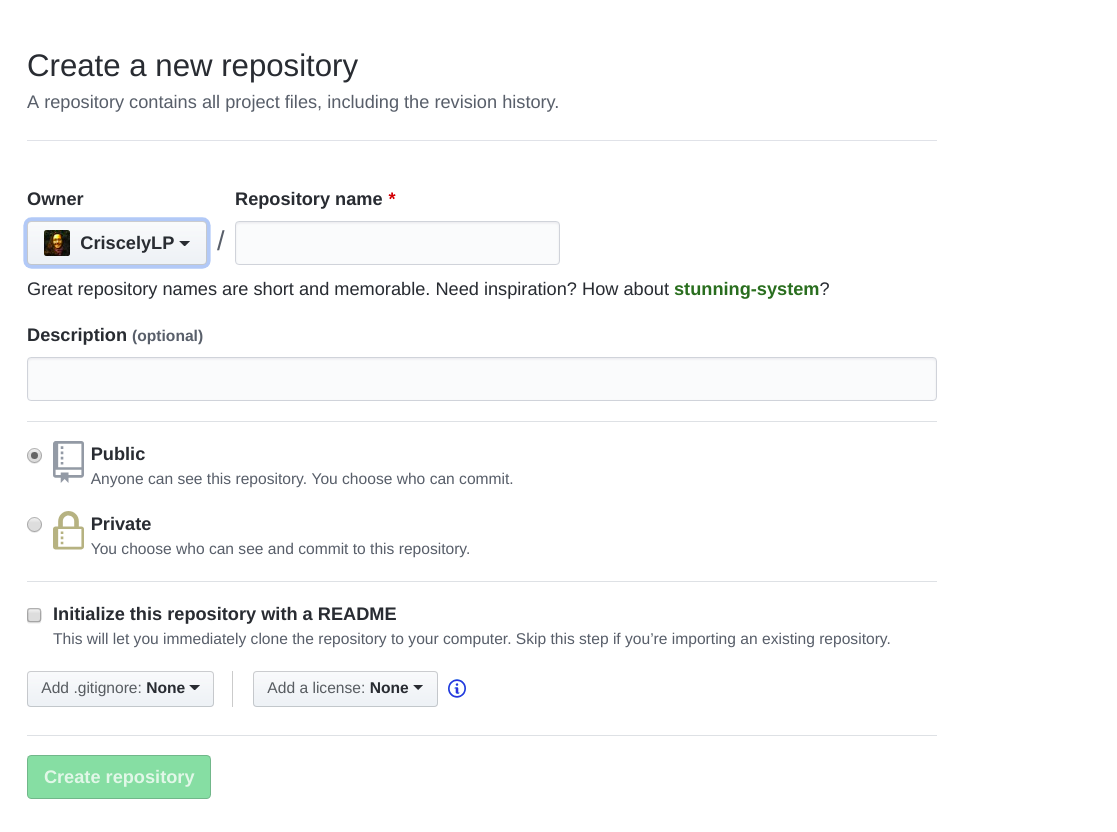
\includegraphics[scale=0.27]{img/github_makeRepo.png}
\end{center}
\end{frame}

\begin{frame}
\frametitle{Exercise 2: Creation of a repository}

\begin{itemize}
     \item Go to your GitHub profile and see the section called Repositories!.
    \item Clone the repository already created (following steps in exercise 1) in your computer!
\end{itemize}
\end{frame}

\begin{frame}[fragile]
\frametitle{Workflow}

Your local repository consists of three trees maintained by git.

\vspace{1em}
\begin{center}
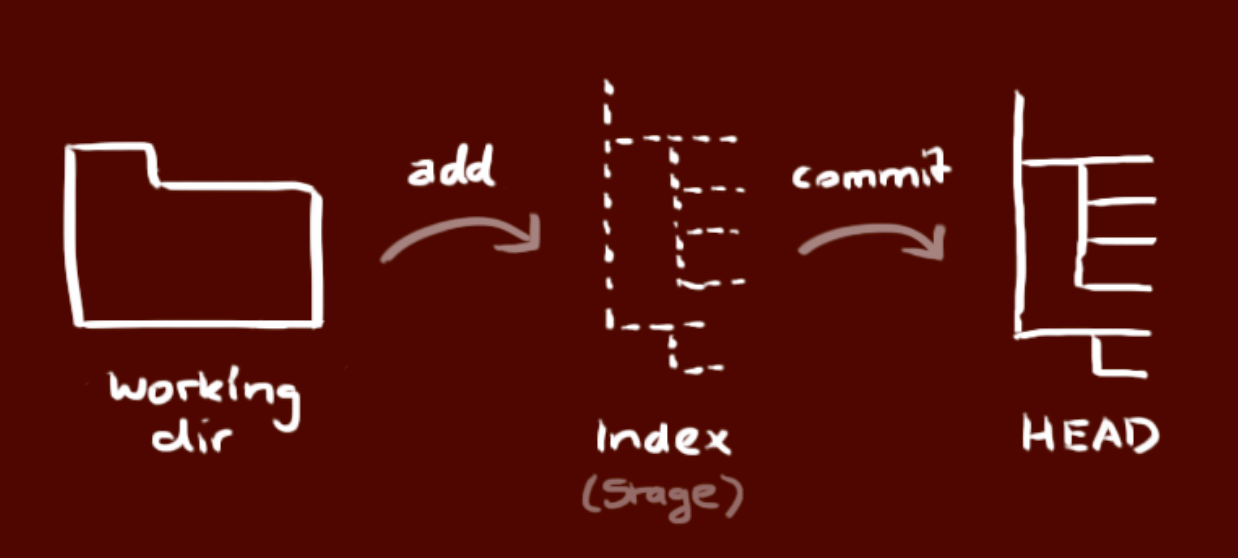
\includegraphics[scale=0.25]{img/workflow.png}
\end{center}
\end{frame}


\begin{frame}[fragile]
\frametitle{Exercise 3: Make changes in the cloned repository}

- After clone the repository on your computer, you are able to make changes using \textbf{add}, \textbf{commit}, and \textbf{push}:
- Create a README.md file (similar to the one in the \verb+git-training+ repo.)
- Now add the file to the distant repository as follows:

\begin{lstlisting}
git add README.md # adding changes for specific file
git commit -m "Commit message" # changes commited to the HEAD
git push origin master #  changes to the remote repository
\end{lstlisting}

- Check the changes in your remote repository.

    \begin{block}{Note}
        To stage all the files of the current directory:
\begin{lstlisting}
git add .
\end{lstlisting}
    \end{block}

\end{frame}

\begin{frame}[fragile]
\frametitle{Exercise 4: Create branches}

- Create a branch from the master one:

\begin{lstlisting}
git checkout -b newbranch
\end{lstlisting}
- Put the branch on GitHub

\begin{lstlisting}
git push origin newbranch
\end{lstlisting}

- Check on the GitHub web page if your branch appears. To check the branches:
\begin{lstlisting}
git branch
\end{lstlisting}

- Edit the README.md file, stage, commit and push changes following the steps of the previous slide. To push on the new branch:
\begin{lstlisting}
git push origin newbranch
\end{lstlisting}

- Check that the file has been updated in the branch.

\end{frame}

\begin{frame}[fragile]
\frametitle{Exercise 5: Merge branches}

Now, the modification provided in the \verb+newbranch+ will be moved back to the main branch.

- Go back to the main branch
\begin{lstlisting}
git checkout master
git branch   # checks that we are on the master branch
\end{lstlisting}

- Merge the newbranch into master
\begin{lstlisting}
git merge newbranch
\end{lstlisting}

- Push the updated master branch
\begin{lstlisting}
git push origin master
\end{lstlisting}

- Remove the newbranch, which is no more usefull
\begin{lstlisting}
git branch -d newbranch   # remove local branch
git push origin --delete newbranch   # remove from distant repo
\end{lstlisting}

\end{frame}


\begin{frame}[fragile]{Managing conflicts}
    - Clone your repository in another location

    - From this new repository, edit the README file and push the change
    
    - Go back to your first repo., edit the README file and push the change. \textbf{You should see an error!}
    
    - Do an update from the distant branch
\begin{lstlisting}
git pull
git status
\end{lstlisting}
    - Resolve conflict, add and commit changes.
    
    - Push the resolved master branch
\begin{lstlisting}
git pull origin master
\end{lstlisting}
\end{frame}

\begin{frame}{See the life of your branches}
    \begin{center}
    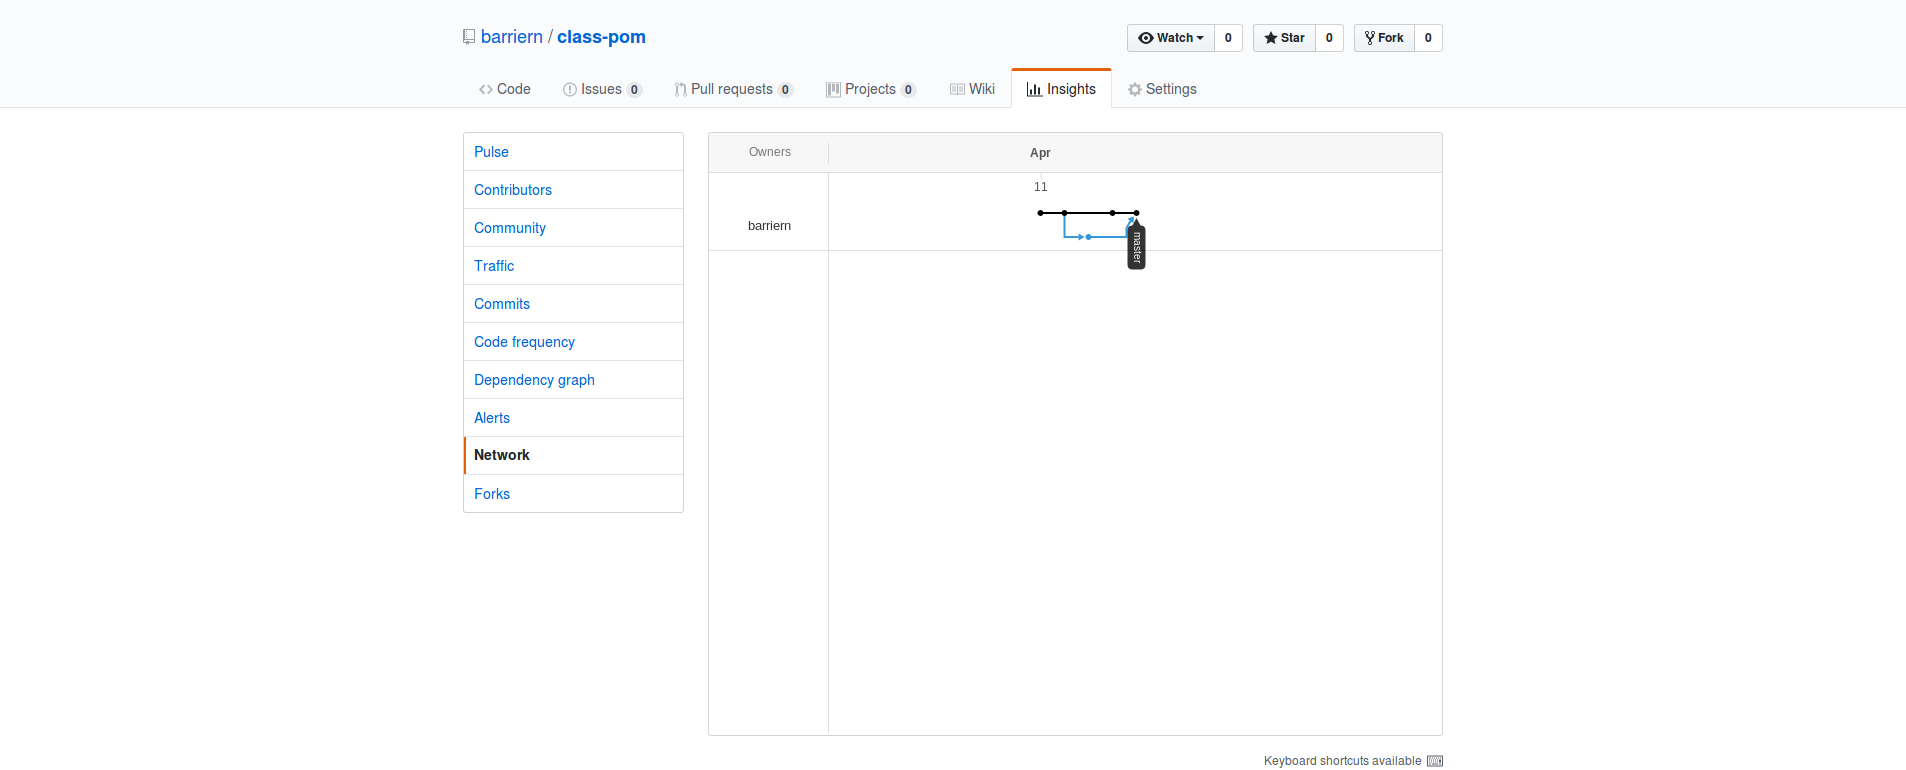
\includegraphics[scale=0.2]{img/network.png}
    \end{center}
\end{frame}

\section{Git Flow (advanced)}

\begin{frame}[fragile]{Git Flow (advanced users)}

    Install the GitFlow extension:

    \begin{lstlisting}[language=bash]
    sudo apt-get install git-flow
    \end{lstlisting}

    \vspace{1em}
    Now, from your directory, initialize the GitFlow workflow:

    \begin{lstlisting}[language=bash]
    git flow init # create the develop branch
    git push origin develop # push the develop branch to the repository
    \end{lstlisting}

\end{frame}

\begin{frame}[fragile]{Creating new features}

    \vspace{-0.5em}

    \begin{lstlisting}
    # recovers the latest develop branch
    git pull origin develop

    # create feature branch from develop and switch to it
    git flow feature start my-feature 

    # put the feature branch to the repo (not necessary)
    git flow feature publish my-feature 

    # edit/add files: new functionalities
    # commit changes to the my-feature branch
    git commit 

    # merge my-feature branch with develop and remove it
    # switch back to develop
    git flow feature finish

    # push updated develop branch
    git push origin develop
    # if conflict (someone has already pushed in develop)
    git pull origin develop
    git push origin develop
    \end{lstlisting}

\end{frame}

\begin{frame}[fragile]{Creating a new release}

    \begin{lstlisting}
    # recovers the latest develop branch
    git pull origin develop

    # create a new release branch
    git flow release start my-release

    # put the release branch to the repo (not necessary)
    git flow release publish my-release 

    # edit/add files: bug fixes + documentation

    # commit changes to the my-feature branch
    git commit 

    # finish the release
    git flow release finish

    # push updated develop/master and tags
    git push origin --tags
    git push origin develop
    git push origin master
    \end{lstlisting}
\end{frame}

\begin{frame}[fragile]
    \frametitle{Creating hotfixes}
    \begin{lstlisting}
    # recovers the latest develop/master branches
    git pull origin develop

    # create a new hotfix branch from master
    # name should be a version name (1.3.2 for instance)
    git flow hotfix start hotfix-tag

    # edit/add files: bug corrections

    # commit changes to the hotfix-tag branch
    git commit 

    # finish the release
    # merge hotfix branch to master/develop
    git flow hotfix finish

    # push updated develop/master and tags
    git push origin --tags
    git push origin develop
    git push origin master
    \end{lstlisting}
\end{frame}

\end{document}
